\documentclass{standalone}
\usepackage{tikz}
\usetikzlibrary{patterns, positioning}


\begin{document}
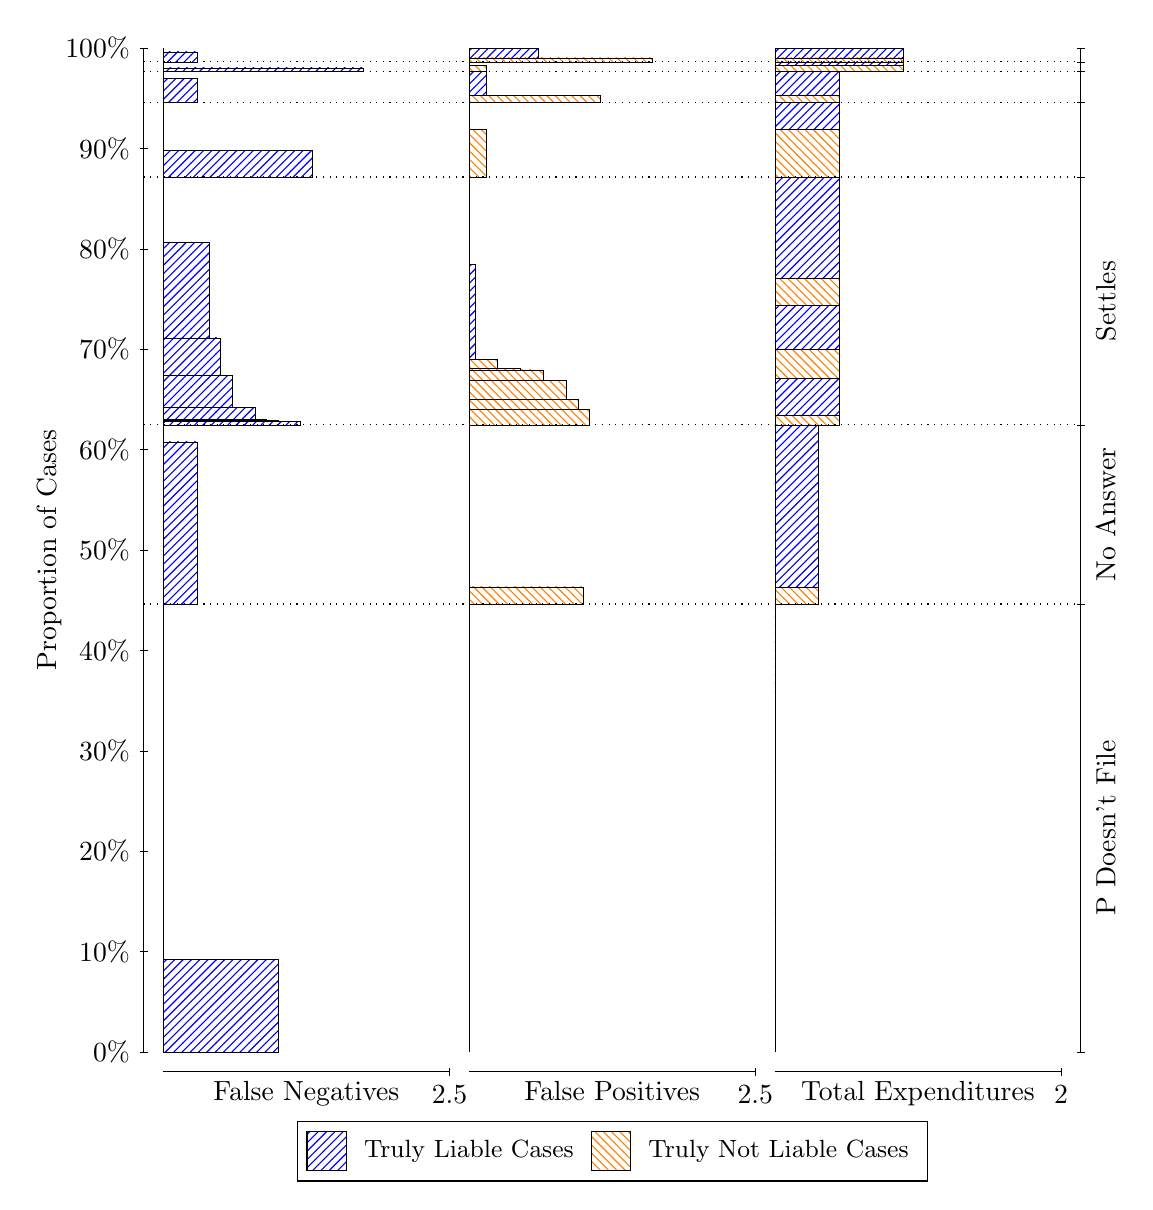
\begin{tikzpicture}
\draw[black, very thin] (1.5,1.75) -- (1.5,14.5);
\node[rotate=90, text=black, anchor=center] at (0.3, 8.125) {Proportion of Cases};
\draw[black, very thin] (1.45,1.75) -- (1.55,1.75);
\node[text=black, anchor=east] at (1.45, 1.75) {0\%};
\draw[black, very thin] (1.45,3.025) -- (1.55,3.025);
\node[text=black, anchor=east] at (1.45, 3.025) {10\%};
\draw[black, very thin] (1.45,4.3) -- (1.55,4.3);
\node[text=black, anchor=east] at (1.45, 4.3) {20\%};
\draw[black, very thin] (1.45,5.575) -- (1.55,5.575);
\node[text=black, anchor=east] at (1.45, 5.575) {30\%};
\draw[black, very thin] (1.45,6.85) -- (1.55,6.85);
\node[text=black, anchor=east] at (1.45, 6.85) {40\%};
\draw[black, very thin] (1.45,8.125) -- (1.55,8.125);
\node[text=black, anchor=east] at (1.45, 8.125) {50\%};
\draw[black, very thin] (1.45,9.4) -- (1.55,9.4);
\node[text=black, anchor=east] at (1.45, 9.4) {60\%};
\draw[black, very thin] (1.45,10.675) -- (1.55,10.675);
\node[text=black, anchor=east] at (1.45, 10.675) {70\%};
\draw[black, very thin] (1.45,11.95) -- (1.55,11.95);
\node[text=black, anchor=east] at (1.45, 11.95) {80\%};
\draw[black, very thin] (1.45,13.225) -- (1.55,13.225);
\node[text=black, anchor=east] at (1.45, 13.225) {90\%};
\draw[black, very thin] (1.45,14.5) -- (1.55,14.5);
\node[text=black, anchor=east] at (1.45, 14.5) {100\%};

\draw[black, very thin] (13.4,1.75) -- (13.4,14.5);
\draw[black, very thin] (13.35,1.75) -- (13.45,1.75);
\node[anchor=west] at (13.35, 1.75) {};
\draw[black, very thin] (13.35,7.4392) -- (13.45,7.4392);
\node[anchor=west] at (13.35, 7.4392) {};
\draw[black, very thin] (13.35,9.7143) -- (13.45,9.7143);
\node[anchor=west] at (13.35, 9.7143) {};
\draw[black, very thin] (13.35,12.862) -- (13.45,12.862);
\node[anchor=west] at (13.35, 12.862) {};
\draw[black, very thin] (13.35,13.807) -- (13.45,13.807);
\node[anchor=west] at (13.35, 13.807) {};
\draw[black, very thin] (13.35,14.2) -- (13.45,14.2);
\node[anchor=west] at (13.35, 14.2) {};
\draw[black, very thin] (13.35,14.324) -- (13.45,14.324);
\node[anchor=west] at (13.35, 14.324) {};
\draw[black, very thin] (13.35,14.5) -- (13.45,14.5);
\node[anchor=west] at (13.35, 14.5) {};

\draw[black, very thin, pattern color=blue, pattern=north east lines] (1.75,1.75) rectangle (3.2033,2.9289);
\draw[black, very thin, pattern color=orange, pattern=north west lines] (1.75,2.9289) rectangle (1.75,7.4392);
\draw[black, very thin, pattern color=blue, pattern=north east lines] (1.75,7.4392) rectangle (2.186,9.4967);
\draw[black, very thin, pattern color=orange, pattern=north west lines] (1.75,9.4967) rectangle (1.75,9.7143);
\draw[black, very thin, pattern color=blue, pattern=north east lines] (1.75,9.7143) rectangle (3.494,9.7542);
\draw[black, very thin, pattern color=blue, pattern=north east lines] (1.75,9.7542) rectangle (3.2033,9.7756);
\draw[black, very thin, pattern color=blue, pattern=north east lines] (1.75,9.7756) rectangle (3.058,9.7863);
\draw[black, very thin, pattern color=blue, pattern=north east lines] (1.75,9.7863) rectangle (2.9127,9.937);
\draw[black, very thin, pattern color=blue, pattern=north east lines] (1.75,9.937) rectangle (2.622,10.346);
\draw[black, very thin, pattern color=blue, pattern=north east lines] (1.75,10.346) rectangle (2.4767,10.82);
\draw[black, very thin, pattern color=blue, pattern=north east lines] (1.75,10.82) rectangle (2.3313,12.035);
\draw[black, very thin, pattern color=orange, pattern=north west lines] (1.75,12.035) rectangle (1.75,12.862);
\draw[black, very thin, pattern color=blue, pattern=north east lines] (1.75,12.862) rectangle (3.6393,13.2);
\draw[black, very thin, pattern color=orange, pattern=north west lines] (1.75,13.2) rectangle (1.75,13.807);
\draw[black, very thin, pattern color=blue, pattern=north east lines] (1.75,13.807) rectangle (2.186,14.11);
\draw[black, very thin, pattern color=orange, pattern=north west lines] (1.75,14.11) rectangle (1.75,14.2);
\draw[black, very thin, pattern color=blue, pattern=north east lines] (1.75,14.2) rectangle (4.2933,14.249);
\draw[black, very thin, pattern color=orange, pattern=north west lines] (1.75,14.249) rectangle (1.75,14.324);
\draw[black, very thin, pattern color=blue, pattern=north east lines] (1.75,14.324) rectangle (2.186,14.451);
\draw[black, very thin, pattern color=orange, pattern=north west lines] (1.75,14.451) rectangle (1.75,14.5);
\draw[black, very thin, pattern color=orange, pattern=north west lines] (5.6333,1.75) rectangle (5.6333,6.2603);
\draw[black, very thin, pattern color=blue, pattern=north east lines] (5.6333,6.2603) rectangle (5.6333,7.4392);
\draw[black, very thin, pattern color=orange, pattern=north west lines] (5.6333,7.4392) rectangle (7.0867,7.6568);
\draw[black, very thin, pattern color=blue, pattern=north east lines] (5.6333,7.6568) rectangle (5.6333,9.7143);
\draw[black, very thin, pattern color=orange, pattern=north west lines] (5.6333,9.7143) rectangle (7.1593,9.914);
\draw[black, very thin, pattern color=orange, pattern=north west lines] (5.6333,9.914) rectangle (7.014,10.035);
\draw[black, very thin, pattern color=orange, pattern=north west lines] (5.6333,10.035) rectangle (6.8687,10.282);
\draw[black, very thin, pattern color=orange, pattern=north west lines] (5.6333,10.282) rectangle (6.578,10.402);
\draw[black, very thin, pattern color=orange, pattern=north west lines] (5.6333,10.402) rectangle (6.4327,10.413);
\draw[black, very thin, pattern color=orange, pattern=north west lines] (5.6333,10.413) rectangle (6.2873,10.434);
\draw[black, very thin, pattern color=orange, pattern=north west lines] (5.6333,10.434) rectangle (5.9967,10.541);
\draw[black, very thin, pattern color=blue, pattern=north east lines] (5.6333,10.541) rectangle (5.706,11.756);
\draw[black, very thin, pattern color=blue, pattern=north east lines] (5.6333,11.756) rectangle (5.6333,12.862);
\draw[black, very thin, pattern color=orange, pattern=north west lines] (5.6333,12.862) rectangle (5.8513,13.468);
\draw[black, very thin, pattern color=blue, pattern=north east lines] (5.6333,13.468) rectangle (5.6333,13.807);
\draw[black, very thin, pattern color=orange, pattern=north west lines] (5.6333,13.807) rectangle (7.3047,13.896);
\draw[black, very thin, pattern color=blue, pattern=north east lines] (5.6333,13.896) rectangle (5.8513,14.2);
\draw[black, very thin, pattern color=orange, pattern=north west lines] (5.6333,14.2) rectangle (5.8513,14.275);
\draw[black, very thin, pattern color=blue, pattern=north east lines] (5.6333,14.275) rectangle (5.6333,14.324);
\draw[black, very thin, pattern color=orange, pattern=north west lines] (5.6333,14.324) rectangle (7.9587,14.374);
\draw[black, very thin, pattern color=blue, pattern=north east lines] (5.6333,14.374) rectangle (6.5053,14.5);
\draw[black, very thin, pattern color=orange, pattern=north west lines] (9.5167,1.75) rectangle (9.5167,6.2603);
\draw[black, very thin, pattern color=blue, pattern=north east lines] (9.5167,6.2603) rectangle (9.5167,7.4392);
\draw[black, very thin, pattern color=orange, pattern=north west lines] (9.5167,7.4392) rectangle (10.062,7.6568);
\draw[black, very thin, pattern color=blue, pattern=north east lines] (9.5167,7.6568) rectangle (10.062,9.7143);
\draw[black, very thin, pattern color=orange, pattern=north west lines] (9.5167,9.7143) rectangle (10.334,9.8349);
\draw[black, very thin, pattern color=blue, pattern=north east lines] (9.5167,9.8349) rectangle (10.334,10.309);
\draw[black, very thin, pattern color=orange, pattern=north west lines] (9.5167,10.309) rectangle (10.334,10.677);
\draw[black, very thin, pattern color=blue, pattern=north east lines] (9.5167,10.677) rectangle (10.334,11.236);
\draw[black, very thin, pattern color=orange, pattern=north west lines] (9.5167,11.236) rectangle (10.334,11.575);
\draw[black, very thin, pattern color=blue, pattern=north east lines] (9.5167,11.575) rectangle (10.334,12.862);
\draw[black, very thin, pattern color=orange, pattern=north west lines] (9.5167,12.862) rectangle (10.334,13.468);
\draw[black, very thin, pattern color=blue, pattern=north east lines] (9.5167,13.468) rectangle (10.334,13.807);
\draw[black, very thin, pattern color=orange, pattern=north west lines] (9.5167,13.807) rectangle (10.334,13.896);
\draw[black, very thin, pattern color=blue, pattern=north east lines] (9.5167,13.896) rectangle (10.334,14.2);
\draw[black, very thin, pattern color=orange, pattern=north west lines] (9.5167,14.2) rectangle (11.152,14.275);
\draw[black, very thin, pattern color=blue, pattern=north east lines] (9.5167,14.275) rectangle (11.152,14.324);
\draw[black, very thin, pattern color=orange, pattern=north west lines] (9.5167,14.324) rectangle (11.152,14.374);
\draw[black, very thin, pattern color=blue, pattern=north east lines] (9.5167,14.374) rectangle (11.152,14.5);
\draw[black, dotted] (1.5,7.4392) -- (13.4,7.4392);
\draw[black, dotted] (1.5,9.7143) -- (13.4,9.7143);
\draw[black, dotted] (1.5,12.862) -- (13.4,12.862);
\draw[black, dotted] (1.5,13.807) -- (13.4,13.807);
\draw[black, dotted] (1.5,14.2) -- (13.4,14.2);
\draw[black, dotted] (1.5,14.324) -- (13.4,14.324);
\draw[black, very thin] (1.75,1.5) -- (5.3833,1.5);
\node[text=black, anchor=north] at (3.5667, 1.5) {False Negatives};
\draw[black, very thin] (5.3833,1.45) -- (5.3833,1.55);
\node[text=black, anchor=north] at (5.3833, 1.45) {2.5};

\draw[black, very thin] (5.6333,1.5) -- (9.2667,1.5);
\node[text=black, anchor=north] at (7.45, 1.5) {False Positives};
\draw[black, very thin] (9.2667,1.45) -- (9.2667,1.55);
\node[text=black, anchor=north] at (9.2667, 1.45) {2.5};

\draw[black, very thin] (9.5167,1.5) -- (13.15,1.5);
\node[text=black, anchor=north] at (11.333, 1.5) {Total Expenditures};
\draw[black, very thin] (13.15,1.45) -- (13.15,1.55);
\node[text=black, anchor=north] at (13.15, 1.45) {2};

\node[text=black, centered, rotate=90] at (13.72, 4.5946) {P Doesn't File};
\node[text=black, centered, rotate=90] at (13.72, 8.5768) {No Answer};
\node[text=black, centered, rotate=90] at (13.72, 11.288) {Settles};





\draw (7.449999999999999,1.5) node[draw=none] (baseCoordinate) {};
\begin{scope}[align=center]
        \matrix[scale=0.5, draw=black, below=0.5cm of baseCoordinate, nodes={draw}, column sep=0.1cm]{
            \node[rectangle, draw, minimum width=0.5cm, minimum height=0.5cm, pattern color=blue, pattern=north east lines] {}; &
            \node[draw=none, font=\small, text=black] (B) {Truly Liable Cases}; &
            \node[rectangle, draw, minimum width=0.5cm, minimum height=0.5cm, pattern color=orange, pattern=north west lines] {}; &
            \node[draw=none, font=\small, text=black] (B) {Truly Not Liable Cases}; \\
            };
\end{scope}

\end{tikzpicture}
\end{document}